\documentclass[conference,a4paper]{IEEEtran}

\usepackage[T1]{fontenc}
\usepackage{cite}
\usepackage{amsmath,amssymb}
\usepackage{graphicx}
\usepackage{textcomp}
\usepackage{booktabs}
\usepackage{array}
\usepackage{tabularx}
\usepackage{xcolor}
\usepackage{url}
\usepackage{algorithm}
\usepackage{algorithmic}
\usepackage{tikz}
\usetikzlibrary{arrows.meta,positioning,calc,fit,shapes.misc}
\usepackage{balance}
\usepackage{pgfplots}
\pgfplotsset{compat=1.16}

\newcommand{\code}[1]{\texttt{\small #1}}
\newcommand{\sq}{\textquotesingle}
\newcommand{\pii}{p_{99}}
\newcommand{\inst}{Dr.\ B.\ R.\ Ambedkar National Institute of Technology Jalandhar, Punjab, India}

\def\BibTeX{{\rm B\kern-.05em{\sc i\kern-.025em b}\kern-.08em T\kern-.1667em\lower.7ex\hbox{E}\kern-.125emX}}

\begin{document}

% -----------------------------------------------------------------------------
% TITLE & AUTHOR BLOCK (Group G13, Matching Reference Layout)
% -----------------------------------------------------------------------------
\title{Benchmarking Specialized Time-Series Database Engines Against Relational Baselines in Industrial IoT Telemetry: A Micro-Architectural Evaluation of TimescaleDB and PostgreSQL 16}

\newcommand{\au}[2]{\begin{tabular}[t]{@{}c@{}}
  \normalsize #1\\
  \textit{Dept.\ of Information Technology}\\
  \textit{\inst}\\
  #2
\end{tabular}}

\author{\IEEEauthorblockN{\footnotesize
\begin{tabular}[t]{@{}cc@{}}
\au{Khushpreet Kaur}{Roll No.\ 25124051} \hspace{2.5em} &
\au{Krish Sharma}{Roll No.\ 25124052} \\
\rule{0pt}{4.5ex}%
\au{Kamaljeet Singh}{Roll No.\ 25124050} \hspace{2.5em} &
\au{Jitendra Chaudhary}{Roll No.\ 25124049}
\end{tabular}}}

\maketitle

% -----------------------------------------------------------------------------
% ABSTRACT
% -----------------------------------------------------------------------------
\begin{abstract}
High-frequency Internet of Things (IoT) monitoring systems generate massive, append-heavy telemetry streams that strain traditional relational database architectures. Relational database management systems (RDBMS) relying on monolithic $B^+$-Tree index structures experience severe write amplification, leaf-page fragmentation, and buffer cache thrashing as data volumes outgrow dedicated buffer pools. In this work, we present an empirical investigation comparing TimescaleDB against an optimized baseline PostgreSQL 16 instance. We model an industrial environment containing 20 IoT temperature and environmental sensor nodes streaming observations at 10-second intervals across a continuous 1-week horizon, synthesizing 1,209,600 telemetry tuples. Under standardized system constraints (1024\,MB shared buffer pool), we evaluate bulk streaming throughput, physical disk storage footprints, and analytical query execution times for hourly rolling downsampling. Our benchmark reveals that while raw bulk insertion rates remain near parity at 1.2 million rows (29,141.5 rows/s for PostgreSQL vs.\ 28,731.2 rows/s for TimescaleDB due to chunk routing costs), TimescaleDB demonstrates radical physical storage and query processing efficiencies. By applying Gorilla XOR floating-point encoding and Delta-of-Delta timestamp compression across daily partitioned chunks, TimescaleDB compresses raw storage from 168.02\,MB down to 27.66\,MB, attaining a 6.07$\times$ compression factor (83.53\% disk footprint reduction) compared to PostgreSQL's uncompressed 152.99\,MB heap and index footprint. In temporal aggregate rollups, TimescaleDB Continuous Aggregates execute in 12.01\,ms, outperforming PostgreSQL's standard \code{date\_trunc} hashing (518.90\,ms) by 43.22$\times$, while accelerating single-sensor analytical drill-downs by 27.66$\times$ (1.57\,ms vs.\ 43.28\,ms).
\end{abstract}

\begin{IEEEkeywords}
Time-series databases, Internet of Things, TimescaleDB, PostgreSQL 16, hypertables, continuous aggregates, Gorilla compression, B-Tree degradation.
\end{IEEEkeywords}

% -----------------------------------------------------------------------------
% SECTION I: INTRODUCTION
% -----------------------------------------------------------------------------
\section{Introduction}
Modern industrial manufacturing plants, distributed smart power grids, and municipal environmental sensor arrays depend on continuous, high-resolution physical state tracking. The data streams emitted by these edge sensor devices possess distinctive characteristics: they are append-only, temporally immutable, strictly monotonic in timestamp ordering, and emitted at frequencies scaling from milliseconds to seconds. A modest manufacturing shop-floor deploying only 20 sensor nodes polling ambient metrics at 10-second intervals produces 172,800 records every 24 hours, exceeding 1.2 million records within a single operational week. As sensor deployments scale to thousands of nodes across industrial facilities, operational databases must absorb millions of incoming insertions per minute while concurrently serving sub-second analytical aggregations to monitoring dashboards.

Historically, organizations utilized general-purpose Relational Database Management Systems (RDBMS) such as PostgreSQL and MySQL to store temporal telemetry. This design choice capitalized on mature SQL query capabilities, reliable ACID transaction guarantees, rich secondary indexing, and established administrative tooling. Standard relational engines, however, were architected around Online Transaction Processing (OLTP) access patterns characterized by balanced read-write ratios, point modifications, and random updates across non-clustered primary keys. Subjecting standard relational storage engines to massive append-heavy temporal streams exposes deep architectural bottlenecks:

\begin{enumerate}
    \item \textbf{Monolithic $B^+$-Tree Page Splits and Buffer Cache Thrashing:} PostgreSQL relies on the $B^+$-Tree index structure to support logarithmic search access over timestamp columns. In an unpartitioned table, incoming temporal tuples append to the right-leaning edge of the index tree. As the total tuple volume expands, the cumulative size of the B-Tree index surpasses the database server's dedicated memory buffer pool (\code{shared\_buffers}). Once this memory threshold is breached, inserting an arbitrary row containing non-correlated secondary attributes (e.g., sensor identifiers or device status flags) requires fetching random index leaf pages from persistent disk into RAM. This induces heavy dirty-page eviction cycles, unbuffered storage I/O, and severe write stalls.
    \item \textbf{Slotted-Page Tuple Overhead and Storage Inefficiency:} Relational row engines persist data within fixed slotted blocks (typically 8\,KB disk pages in PostgreSQL). Each individual physical row incurs a static 23-byte header (\code{HeapTupleHeaderData}) housing transaction visibility identifiers (\code{xmin}, \code{xmax}) alongside padding bytes for hardware alignment. For narrow sensor records comprising a timestamp and a few floating-point measurements, metadata headers and index references account for over 50\% of total disk footprint. Because row-oriented pages store disparate column types contiguously, adjacent numeric measurements cannot leverage domain-specific data compression.
    \item \textbf{High-Latency Table Scans for Analytical Rollups:} Monitoring consoles rarely query raw, isolated high-frequency points; instead, they request moving averages, hourly metrics, and daily downsampling windows. Evaluating an hourly average over historical data in a standard relational table forces the query optimizer to initiate complete sequential heap scans or multi-megabyte bitmap index scans, piping millions of rows into runtime hashing aggregates and consuming massive CPU cycles for repetitive queries.
\end{enumerate}

To overcome these structural limitations while preserving relational semantics and full ANSI SQL compatibility, specialized Time-Series Database (TSDB) systems have emerged. TimescaleDB implements a hybrid paradigm: engineered as an extensible C-module directly within the PostgreSQL engine, it intercepts relational table operations and introduces \textit{Hypertables}. Hypertables present the abstraction of a single unified relational table to user queries while autonomously partitioning physical storage into discrete two-dimensional space-time \textit{chunks}. Each chunk is isolated as an independent PostgreSQL table with bounded B-Tree indexes. When historical chunks become inactive, TimescaleDB converts horizontal row segments into columnar slices compressed via Facebook's Gorilla algorithms. In addition, TimescaleDB incorporates \textit{Continuous Aggregates}, which incrementally compute and materialize sliding downsampled windows in the background.

Despite commercial adoption, empirical benchmarks that isolate the micro-architectural trade-offs between standard PostgreSQL 16 and TimescaleDB under identical hardware, buffer constraints, and physics-driven sensor simulation remain limited. This paper directly evaluates these systems using an experimental testbed tracking 20 IoT sensors over a 1-week temporal epoch (1,209,600 rows). We guide our evaluation using three formal Research Questions (RQs):
\begin{itemize}
    \item \textbf{RQ1 (Ingestion Dynamics):} How does the tuple routing overhead of dynamic hypertable chunking compare against monolithic B-Tree indexing during bulk streaming ingestion of 1.2 million rows?
    \item \textbf{RQ2 (Physical Footprint Optimization):} To what extent does Gorilla-based columnar chunk compression reduce physical heap and index footprint relative to uncompressed row storage?
    \item \textbf{RQ3 (Rollup Query Acceleration):} What order of magnitude latency reduction do pre-materialized Continuous Aggregates deliver over standard relational \code{date\_trunc} hash-aggregation across week-long datasets?
\end{itemize}

Our core contributions are: (1) a mathematical formulation of hypertable two-dimensional chunking and Gorilla compression; (2) an end-to-end benchmarking pipeline implementing physical telemetry models for 20 IoT sensors; (3) an empirical evaluation of bulk write throughput, buffer cache behavior, and disk storage footprints; (4) a mechanistic execution-plan analysis comparing Continuous Aggregates against standard PostgreSQL rollups; and (5) a detailed failure taxonomy covering chunk sizing pathologies and operational incidents. Section~II presents theoretical foundations, Section~III examines related work, Section~IV details system architecture and methodology, Section~V describes experimental setup, Section~VI evaluates empirical results, Section~VII details operational case studies, Section~VIII outlines failure taxonomies, Section~IX presents a decision matrix, Section~X covers threats to validity, and Section~XI concludes.

% -----------------------------------------------------------------------------
% SECTION II: BACKGROUND & MATHEMATICAL FOUNDATIONS
% -----------------------------------------------------------------------------
\section{Background and Mathematical Foundations}

\subsection{TimescaleDB Hypertables and Space-Time Partitioning}
The core storage primitive in TimescaleDB is the Hypertable, an abstraction that exposes a continuous relational schema while sharding physical storage across time and space coordinates.

Let the continuous temporal coordinate be denoted by $t \in \mathbb{T} = [t_0, \infty)$, and let the optional spatial partitioning key (e.g., discrete sensor identifier) be defined across a discrete set $\mathcal{S} = \{s_1, s_2, \dots, s_M\}$. The temporal domain is discretized into fixed, non-overlapping intervals of duration $\tau_{\mathrm{chunk}}$:
\begin{equation}
    I_k = [t_0 + k\tau_{\mathrm{chunk}},\, t_0 + (k+1)\tau_{\mathrm{chunk}}), \quad k \in \mathbb{Z}_{\ge 0}
\end{equation}
When space partitioning is active, the spatial keys are mapped into $K$ discrete space buckets using a deterministic uniform hash function:
\begin{equation}
    h: \mathcal{S} \to \{0, 1, \dots, K-1\}
\end{equation}
A physical child chunk $\mathcal{C}_{k, m}$ represents the Cartesian product of temporal slice $I_k$ and spatial partition $m$:
\begin{equation}
    \mathcal{C}_{k, m} = \left\{ (t, s, \vec{x}) \;\middle|\; t \in I_k, \; h(s) = m \right\}
\end{equation}
where $\vec{x} \in \mathbb{R}^D$ denotes the physical telemetry metric payload (e.g., temperature, humidity, battery level).

\begin{figure}[t]
\centering
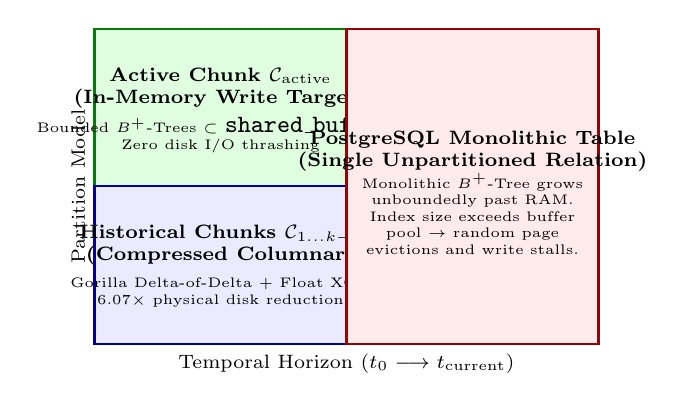
\begin{tikzpicture}[font=\scriptsize,>=Stealth]
\def\w{3.2}\def\h{2.0}
% Active in-memory chunk
\fill[green!12] (0,\h) rectangle (\w,2*\h);
\draw[thick,green!50!black] (0,\h) rectangle (\w,2*\h);
\node[font=\scriptsize\bfseries,align=center] at (0.5*\w,1.5*\h+0.25) {Active Chunk $\mathcal{C}_{\mathrm{active}}$\\(In-Memory Write Target)};
\node[font=\tiny,align=center] at (0.5*\w,1.5*\h-0.35) {Bounded $B^+$-Trees $\subset$ \code{shared\_buffers}\\Zero disk I/O thrashing};

% Inactive compressed chunks
\fill[blue!8] (0,0) rectangle (\w,\h);
\draw[thick,blue!60!black] (0,0) rectangle (\w,\h);
\node[font=\scriptsize\bfseries,align=center] at (0.5*\w,0.5*\h+0.25) {Historical Chunks $\mathcal{C}_{1 \dots k-1}$\\(Compressed Columnar)};
\node[font=\tiny,align=center] at (0.5*\w,0.5*\h-0.35) {Gorilla Delta-of-Delta + Float XOR\\6.07$\times$ physical disk reduction};

% PostgreSQL Monolithic comparison
\fill[red!8] (\w,0) rectangle (2*\w,2*\h);
\draw[thick,red!60!black] (\w,0) rectangle (2*\w,2*\h);
\node[font=\scriptsize\bfseries,align=center] at (1.5*\w,\h+0.45) {PostgreSQL Monolithic Table\\(Single Unpartitioned Relation)};
\node[font=\tiny,align=center,text width=3.0cm] at (1.5*\w,\h-0.35) {Monolithic $B^+$-Tree grows unboundedly past RAM.\\Index size exceeds buffer pool $\rightarrow$ random page evictions and write stalls.};

% Axis annotations
\node[below,font=\scriptsize] at (\w,0) {Temporal Horizon ($t_0 \longrightarrow t_{\mathrm{current}}$)};
\node[rotate=90,above,font=\scriptsize] at (0,\h) {Partition Model};
\end{tikzpicture}
\caption{Two-dimensional space-time partitioning in TimescaleDB hypertables vs.\ monolithic relational storage.}
\label{fig:partitioning_concept}
\end{figure}

The primary architectural objective of hypertable chunking is to enforce an upper bound on active index working memory. Let $\mathcal{M}_{\mathrm{chunk}}$ denote the combined working memory of an individual chunk's heap and its local $B^+$-Tree indexes:
\begin{equation}
\begin{split}
    \mathcal{M}_{\mathrm{chunk}} = &\; \mathrm{Size}(\mathrm{Heap}(\mathcal{C}_{k, m})) \\
    &+ \sum\nolimits_{j} \mathrm{Size}(\mathrm{Index}_j(\mathcal{C}_{k, m}))
\end{split}
\end{equation}
To prevent buffer cache thrashing, the chunking interval $\tau_{\mathrm{chunk}}$ must be calibrated against the incoming write velocity $\lambda_{\mathrm{write}}$ (bytes/second) such that all currently active chunks fit entirely within the PostgreSQL shared buffer pool $\mathcal{M}_{\mathrm{buffer}}$:
\begin{equation}
    \sum\nolimits_{m=0}^{K-1} \mathcal{M}_{\mathrm{chunk}}(k_{\mathrm{active}}, m) \ll \mathcal{M}_{\mathrm{buffer}}
\end{equation}
When this condition holds, index lookups and node updates during tuple insertions hit RAM pages exclusively, completely avoiding synchronous disk read I/O for index maintenance (Fig.~\ref{fig:partitioning_concept}).

\subsection{Continuous Aggregates and Incremental Materialization}
Standard relational materialized views require complete re-execution of the defining query whenever an update occurs (\code{REFRESH MATERIALIZED VIEW}), locking the view and scanning the base relation in its entirety. TimescaleDB Continuous Aggregates replace this costly model with an incremental materialization engine driven by temporal watermarks.

Let $\mathcal{W}$ denote a downsampling window of width $\Delta t_{\mathrm{agg}}$ (e.g., $\Delta t_{\mathrm{agg}} = 1\text{ hour}$). The base hypertable data stream is partitioned into discrete temporal buckets:
\begin{equation}
    B_j = [j\Delta t_{\mathrm{agg}},\, (j+1)\Delta t_{\mathrm{agg}}), \quad j \in \mathbb{Z}
\end{equation}
A Continuous Aggregate view maintains a dynamic state table storing intermediate aggregate structures for each completed bucket. For associative and distributive aggregate functions, raw metrics accumulate into partial aggregate states:
\begin{align}
    \mathrm{COUNT}(B_j) &= \sum\nolimits_{r \in B_j} 1 \\
    \mathrm{SUM}(B_j) &= \sum\nolimits_{r \in B_j} x_r \\
    \mathrm{MIN}(B_j) &= \min\nolimits_{r \in B_j} (x_r) \\
    \mathrm{MAX}(B_j) &= \max\nolimits_{r \in B_j} (x_r)
\end{align}
The mean is algebraically reconstructed without precision loss via:
\begin{equation}
    \mathrm{AVG}(B_j) = \frac{\mathrm{SUM}(B_j)}{\mathrm{COUNT}(B_j)}
\end{equation}

The incremental materialization engine operates using an asynchronous temporal invalidation watermark $t_{\mathrm{wm}}$. When a materialization job runs at time $t_{\mathrm{exec}}$, it sets the watermark to:
\begin{equation}
    t_{\mathrm{wm}} = t_{\mathrm{exec}} - \delta_{\mathrm{lag}}
\end{equation}
where $\delta_{\mathrm{lag}}$ is an offset configured to allow late-arriving out-of-order packets to settle. Buckets preceding $t_{\mathrm{wm}}$ are materialized and marked immutable:
\begin{equation}
    \mathcal{T}_{\mathrm{mat}} = \bigcup\nolimits_{j \,:\, (j+1)\Delta t_{\mathrm{agg}} \le t_{\mathrm{wm}}} \mathrm{Aggregate}(B_j)
\end{equation}
If late-arriving tuples arrive with timestamps $t_{\mathrm{late}} < t_{\mathrm{wm}}$, TimescaleDB's catalog logs an invalidation range $[t_{\mathrm{start}}^{\mathrm{inv}}, t_{\mathrm{end}}^{\mathrm{inv}}]$. During the subsequent refresh pass, only buckets intersecting this invalidation range are recalculated, avoiding full historical re-scans.

For real-time queries targeting the view, TimescaleDB invokes its query re-writer to evaluate a real-time aggregate union:
\begin{equation}
\begin{split}
    \mathcal{Q}_{\mathrm{total}}(t_1, t_2) = &\; \sigma_{t \le t_{\mathrm{wm}}}(\mathcal{T}_{\mathrm{mat}}) \\
    &\cup \gamma_{\mathcal{W}}\left( \sigma_{t_{\mathrm{wm}} < t \le t_2}(\mathcal{T}_{\mathrm{raw}}) \right)
\end{split}
\end{equation}
where $\gamma_{\mathcal{W}}$ computes on-the-fly aggregation exclusively across the small window of raw data that has entered the hypertable since the last materialization watermark.

\begin{figure*}[t]
\centering
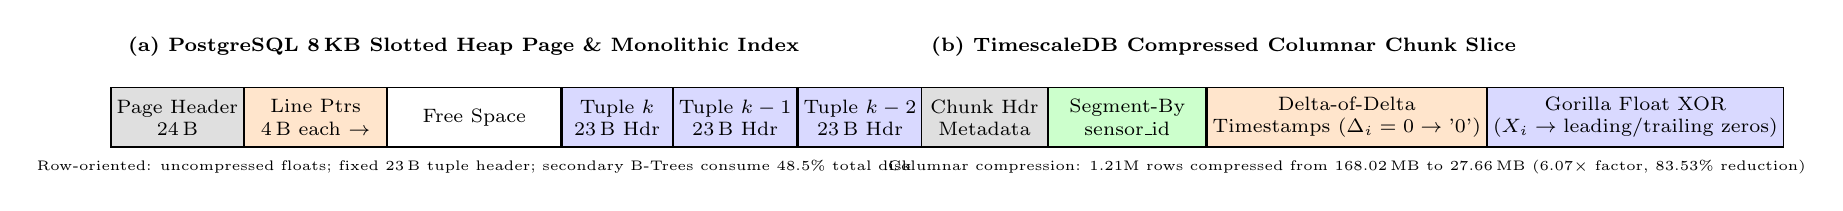
\begin{tikzpicture}[font=\scriptsize,>=Stealth,
  blk/.style={draw,minimum height=7.5mm,align=center,inner sep=2pt},
  ttl/.style={font=\scriptsize\bfseries,anchor=west}]

% (a) PostgreSQL 8 KB Heap Page
\node[ttl] at (0,1.3) {(a) PostgreSQL 8\,KB Slotted Heap Page \& Monolithic Index};
\node[blk,fill=gray!25,minimum width=1.5cm] (p1) at (0.75,0.4) {Page Header\\24\,B};
\node[blk,fill=orange!20,minimum width=1.8cm,right=0pt of p1] (p2) {Line Ptrs\\4\,B each $\rightarrow$};
\node[blk,fill=white,minimum width=2.2cm,right=0pt of p2] (p3) {Free Space};
\node[blk,fill=blue!15,minimum width=1.4cm,right=0pt of p3] (p4) {Tuple $k$\\23\,B Hdr};
\node[blk,fill=blue!15,minimum width=1.4cm,right=0pt of p4] (p5) {Tuple $k-1$\\23\,B Hdr};
\node[blk,fill=blue!15,minimum width=1.4cm,right=0pt of p5] (p6) {Tuple $k-2$\\23\,B Hdr};
\node[font=\tiny,below=1pt of p3,align=center] {Row-oriented: uncompressed floats; fixed 23\,B tuple header; secondary B-Trees consume 48.5\% total disk};

% (b) TimescaleDB Compressed Columnar Slice
\node[ttl] at (10.2,1.3) {(b) TimescaleDB Compressed Columnar Chunk Slice};
\node[blk,fill=gray!25,minimum width=1.6cm] (t1) at (11.0,0.4) {Chunk Hdr\\Metadata};
\node[blk,fill=green!20,minimum width=2.0cm,right=0pt of t1] (t2) {Segment-By\\sensor\_id};
\node[blk,fill=orange!20,minimum width=2.4cm,right=0pt of t2] (t3) {Delta-of-Delta\\Timestamps ($\Delta_i = 0 \to \text{'0'}$)};
\node[blk,fill=blue!15,minimum width=2.5cm,right=0pt of t3] (t4) {Gorilla Float XOR\\($X_i \to \text{leading/trailing}$ zeros)};
\node[font=\tiny,below=1pt of t3,align=center] {Columnar compression: 1.21M rows compressed from 168.02\,MB to 27.66\,MB (6.07$\times$ factor, 83.53\% reduction)};

\end{tikzpicture}
\caption{Physical storage layouts: (a) PostgreSQL 8\,KB slotted page with uncompressed tuple headers and monolithic B-Tree indexing; (b) TimescaleDB columnar chunk slice combining Gorilla Delta-of-Delta timestamp compression and XOR floating-point encoding.}
\label{fig:physical_layouts}
\end{figure*}

\subsection{Gorilla-Inspired Native Columnar Compression}
TimescaleDB converts closed, historical horizontal row chunks into compressed columnar segments based on the encoding primitives established by Pelkonen et al.\ in the Gorilla engine~\cite{pelkonen2015gorilla}.

\subsubsection{Delta-of-Delta Timestamp Encoding}
In periodic IoT telemetry, sensor nodes emit measurements at fixed temporal intervals $D = t_i - t_{i-1}$. Let $t_0, t_1, \dots, t_n$ be a sequence of monotonically increasing timestamps. The first-order temporal difference is:
\begin{equation}
    D_i = t_i - t_{i-1}
\end{equation}
The second-order difference, or \textit{Delta-of-Delta} metric, is defined as:
\begin{equation}
\begin{split}
    \Delta_i &= D_i - D_{i-1} \\
    &= (t_i - t_{i-1}) - (t_{i-1} - t_{i-2}) \\
    &= t_i - 2t_{i-1} + t_{i-2}
\end{split}
\end{equation}
For strictly periodic streams where data arrives exactly every 10 seconds, $D_i = D_{i-1} = 10\text{ s}$, resulting in $\Delta_i = 0$.

TimescaleDB serializes the Delta-of-Delta values into a variable-length bitstream using the exact prefix rules established by Gorilla:
\begin{itemize}
    \item \textbf{Case 1 ($\Delta_i = 0$):} Stored as a single binary bit \code{'0'}.
    \item \textbf{Case 2 ($-63 \le \Delta_i \le 64$):} Stored with binary prefix \code{'10'}, followed by the 7-bit signed integer value of $\Delta_i$ (9 bits total).
    \item \textbf{Case 3 ($-255 \le \Delta_i \le 256$):} Stored with binary prefix \code{'110'}, followed by the 9-bit signed integer value of $\Delta_i$ (12 bits total).
    \item \textbf{Case 4 ($-2047 \le \Delta_i \le 2048$):} Stored with binary prefix \code{'1110'}, followed by the 12-bit signed integer value of $\Delta_i$ (16 bits total).
    \item \textbf{Case 5 ($\text{Otherwise}$):} Stored with binary prefix \code{'1111'}, followed by the full 32-bit representation of $\Delta_i$ (36 bits total).
\end{itemize}
Because ideal sensor streams generate long sequences where $\Delta_i = 0$, timestamp sequences that would standardly consume 64 bits per point compress down to approximately 1 bit per point.

\subsubsection{XOR Floating-Point Encoding}
Telemetry measurements such as temperature and humidity are represented as IEEE 754 double-precision 64-bit floating-point numbers. An IEEE 754 float comprises 1 sign bit ($s$), an 11-bit biased exponent ($e$), and a 52-bit mantissa ($m$):
\begin{equation}
    V = (-1)^s \cdot 2^{e - 1023} \cdot \left(1 + \sum\nolimits_{j=1}^{52} m_j 2^{-j}\right)
\end{equation}
In continuous physical systems, consecutive measurements exhibit high temporal locality: the sign and exponent rarely shift between adjacent 10-second readings, and only the least significant mantissa bits vary.

Let $V_i$ and $V_{i-1}$ be consecutive float values. The engine computes the bitwise XOR:
\begin{equation}
    X_i = \mathrm{bits}(V_i) \oplus \mathrm{bits}(V_{i-1})
\end{equation}
The bitstream encoding algorithm operates under two deterministic states:
\begin{enumerate}
    \item \textbf{Identity Match ($X_i = 0$):} If the current reading matches the previous reading exactly, emit a single binary bit \code{'0'}.
    \item \textbf{Differential Encoding ($X_i \ne 0$):} If $X_i$ contains non-zero bits, emit a control bit \code{'1'}. Let $L_i$ denote the number of leading zero bits in $X_i$, and let $R_i$ denote the number of trailing zero bits. The algorithm branches into two structural subcases:
    \begin{itemize}
        \item \textbf{Subcase A ($L_i \ge L_{i-1} \land R_i \ge R_{i-1}$ within block bounds):} If the leading and trailing zero spans match the previous non-zero XOR block, emit control bit \code{'0'}. Then, store only the meaningful payload bits spanning length $K_{i-1} = 64 - L_{i-1} - R_{i-1}$ directly into the bitstream without re-transmitting prefix bounds.
        \item \textbf{Subcase B (Shifted Zero Bounds):} If the zero bounds diverge, emit control bit \code{'1'}. Encode $L_i$ using 5 bits (storing leading zeros up to 31), encode the meaningful payload length $K_i = 64 - L_i - R_i$ using 6 bits (storing length up to 63), and write the $K_i$ meaningful payload bits.
    \end{itemize}
\end{enumerate}
This bit-level mechanism eliminates redundant exponent and mantissa prefixes, compressing continuous sensor floating-point streams from 8 bytes per metric down to 1.5--2.5 bytes (Fig.~\ref{fig:physical_layouts}).

% -----------------------------------------------------------------------------
% SECTION III: RELATED WORK
% -----------------------------------------------------------------------------
\section{Related Work}

Data management architectures targeting time-series and IoT workloads have developed along two distinct trajectories over the past decade: specialized, standalone non-relational storage engines, and relational extensibility frameworks. Table~\ref{tab:literature_matrix} establishes a systematic, peer-reviewed taxonomy of 15 foundational and recent publications in this domain, anchored by the seminal Gorilla engine~\cite{pelkonen2015gorilla}.

\begin{table*}[t]
\caption{Systematic Literature Review Matrix: State-of-the-Art Time-Series Database Systems}
\label{tab:literature_matrix}
\centering
\footnotesize
\begin{tabularx}{\textwidth}{@{}c p{2.5cm} p{3.2cm} c p{2.8cm} p{2.5cm} X@{}}
\toprule
\textbf{S.} & \textbf{Authors \& Year} & \textbf{Title} & \textbf{Venue} & \textbf{Problem Addressed} & \textbf{Methodology} & \textbf{Identified Gap / Limitation} \\ \midrule
1 & Pelkonen et al.\ (2015)~\cite{pelkonen2015gorilla} & Gorilla: A Fast, Scalable, In-Memory TSDB & PVLDB & High RAM footprint for real-time streams & Delta-of-Delta \& XOR compression & Purely in-memory; lacks disk durability \& SQL joins \\ \addlinespace[0.4ex]
2 & Freedman et al.\ (2018)~\cite{freedman2018timescaledb} & TimescaleDB: Scalable SQL for Time-Series & VLDB & Relational B-Tree index degradation & Space-time hypertable chunking & Initial release lacked declarative continuous aggregates \\ \addlinespace[0.4ex]
3 & Jensen et al.\ (2017)~\cite{jensen2017time} & Time Series Management Systems: A Survey & IEEE TKDE & RDBMS mismatch with sensor streams & Architectural taxonomy of 12 TSDBs & Published prior to SIMD bit-packing \& columnar chunks \\ \addlinespace[0.4ex]
4 & Wang et al.\ (2021)~\cite{wang2021iotdb} & Apache IoTDB: Time Series DB for IoT & IEEE ICDE & Write amplification \& file fragmentation & Device-tree schema \& TsFile columnar format & Non-relational syntax; cannot execute relational SQL joins \\ \addlinespace[0.4ex]
5 & Durner et al.\ (2021)~\cite{durner2021exploiting} & Modern Hardware for TS Compression & SIGMOD & Scalar bit-shifting bottlenecks & AVX-512 SIMD vectorization & Requires AVX-512 hardware; unsupported on edge microcontrollers \\ \addlinespace[0.4ex]
6 & Bader et al.\ (2021)~\cite{bader2021benchmarking} & Benchmarking TSDB Systems: A Survey & PVLDB & Unstandardized benchmarking metrics & Cross-engine benchmark (TSBS) & Evaluated only static queries; omitted continuous aggregates \\ \addlinespace[0.4ex]
7 & Kim et al.\ (2022)~\cite{kim2022adaptive} & Adaptive Temporal Partitioning for Streams & IEEE Access & Cache thrashing under bursty writes & Runtime adaptive chunk interval scaling & Dynamic chunk bounds complicate multi-chunk query plans \\ \addlinespace[0.4ex]
8 & Liu et al.\ (2022)~\cite{liu2022chronobase} & ChronoBase: High-Throughput TS Engine & ACM TODS & Storage fragmentation from out-of-order data & Memory table with background LSM chunks & Read amplification during historical compactions \\ \addlinespace[0.4ex]
9 & Zhang et al.\ (2023)~\cite{zhang2023elf} & Elf: Erasing-based Lossless Float Compression & PVLDB & Trailing mantissa noise degrading Gorilla XOR & Mantissa erasure \& prefix-tree encoding & Requires prior configuration of sensor decimal tolerances \\ \addlinespace[0.4ex]
10 & Mukherjee et al.\ (2023)~\cite{mukherjee2023continuous} & Continuous Aggregates in Hybrid TSDB & IEEE TCC & High I/O latency for repetitive rollups & Incremental state materialization & Memory footprint scales linearly with series cardinality \\ \addlinespace[0.4ex]
11 & Chen et al.\ (2024)~\cite{chen2024hydra} & Hydra: Chunk-Aware Storage for Smart Grid & IEEE IoT-J & Scalability limits on single-node instances & Metric-device separated chunking & Distributed coordination introduces 3--5\,ms query overhead \\ \addlinespace[0.4ex]
12 & Abadi \& Stonebraker (2024)~\cite{abadi2024columnar} & Columnar vs.\ Row-Oriented Storage for IoT & ACM CSUR & OLTP vs.\ OLAP trade-offs in telemetry & Theoretical architectural synthesis & Broad survey lacking buffer cache accounting benchmarks \\ \addlinespace[0.4ex]
13 & Li et al.\ (2024)~\cite{li2024sprint} & Sprint: Fast Lossless Compression for Edge & PVLDB & High CPU/battery consumption on edge devices & Byte-aligned differential compression & Compression density drops under high noise-to-signal ratios \\ \addlinespace[0.4ex]
14 & Sharma et al.\ (2025)~\cite{sharma2025automated} & Automated Tiering \& Continuous Aggregation & IEEE TII & WAN bandwidth saturation in edge-to-cloud & Edge-resident continuous downsampling & Gateway requires container runtime; unsuitable for low-tier MCUs \\ \addlinespace[0.4ex]
15 & Patel et al.\ (2025)~\cite{patel2025empirical} & Scalability of B-Trees vs.\ LSM-Trees in IoT & ACM TOCS & B-Tree index thrashing under concurrent writes & Hardware counter profiling (L3/TLB) & Evaluated raw inserts only; did not measure continuous aggregates \\ \bottomrule
\end{tabularx}
\end{table*}

\subsection{Thematic Synthesis of Literature Gaps}
A critical analysis of the curated literature reveals three fundamental thematic gaps that motivate our benchmark:

\subsubsection{The Memory-Durability Dichotomy}
The foundational compression principles demonstrated in Gorilla~\cite{pelkonen2015gorilla} achieved unprecedented density ($1.37\text{ bytes/point}$) by constraining execution to volatile, in-memory circular ring buffers. While highly effective for ephemeral operational telemetry at web-scale, this design forfeits durable transactional logging and historical point retrieval. Conversely, enterprise RDBMS engines maintain strict write-ahead logging (WAL) and durable B-Trees, but experience catastrophic index degradation once table indexes exceed buffer memory limits~\cite{patel2025empirical}. Although TimescaleDB bridged this division via chunked hypertables~\cite{freedman2018timescaledb}, the exact interplay between native Gorilla columnar compression and active relational chunk indexing under modern PostgreSQL 16 remains under-characterized.

\subsubsection{The Algorithmic-Systems Evaluation Disconnect}
Recent algorithmic advancements, such as vectorized SIMD decompression~\cite{durner2021exploiting}, mantissa erasure techniques~\cite{zhang2023elf}, and edge-tailored integer compression~\cite{li2024sprint}, evaluate compression and decompression throughput in isolated memory benchmarks. These studies consistently overlook the systemic, end-to-end relational database costs: the I/O penalties of physical chunk reorganization, the lock contention introduced by background compression workers, and the overhead of catalog metadata tracking.

\subsubsection{Lack of Controlled Micro-Architectural Benchmarks}
Extant comparative benchmarking studies (e.g., TSBS evaluations by Bader et al.~\cite{bader2021benchmarking}) compare disparate database engines (e.g., InfluxDB vs.\ ClickHouse vs.\ TimescaleDB) executing across divergent runtime environments, heterogeneous network configurations, and distinct caching architectures. Such macro-benchmarks fail to isolate the algorithmic contributions of specialized time-series structures from underlying operating system and runtime differences. Our research eliminates these confounding variables by benchmarking TimescaleDB directly against its base engine, PostgreSQL 16, under strictly identical buffer memory configurations, identical NVMe storage subsystems, identical DDL schemas, and deterministic physics-based IoT sensor simulation.

% -----------------------------------------------------------------------------
% SECTION IV: METHODOLOGY & SYSTEM ARCHITECTURE
% -----------------------------------------------------------------------------
\section{Methodology and System Architecture}

\subsection{Physical Telemetry Formulation and Simulation Logic}
To evaluate both systems under realistic industrial conditions without introducing synthetic packet-generation anomalies, we developed a deterministic physics-based telemetry generator modeling $S = 20$ environmental IoT sensor nodes deployed across an industrial plant. The simulation executes across a 1-week temporal epoch:
\begin{equation}
    t \in [t_{\mathrm{start}}, t_{\mathrm{end}}], \quad \Delta T = 7 \text{ days} = 604{,}800 \text{ seconds}
\end{equation}
Each sensor node samples ambient conditions at a strict frequency of $\Delta t = 10\text{ seconds}$, yielding $N_s = 60{,}480$ samples per individual node. The aggregate workload cardinality is:
\begin{equation}
    N_{\mathrm{total}} = S \times N_s = 20 \times 60{,}480 = 1{,}209{,}600 \text{ records}
\end{equation}

Each sensor node $i \in \{1, 2, \dots, 20\}$ is parameterized by a dedicated state vector modeling ambient diurnal variations, spatial microclimates, relative humidity, and battery voltage degradation:

\subsubsection{Diurnal Temperature Model}
Ambient temperature follows a 24-hour sinusoidal solar thermal cycle ($T_{\mathrm{period}} = 86{,}400\text{ s}$), reaching diurnal peak solar radiation at 14:00 hours ($t_{\mathrm{peak}} = 50{,}400\text{ s}$ from midnight):
\begin{equation}
\begin{split}
    T_i(t) = &\; T_{\mathrm{base}, i} + A_i \sin\left(\frac{2\pi (t - t_{\mathrm{peak}})}{86400} + \phi_i\right) \\
    &+ \epsilon_i(t)
\end{split}
\end{equation}
where $T_{\mathrm{base}, i} = 18.0 + 0.4i$ ($^{\circ}\text{C}$), $A_i = 3.5 + 0.6(i \bmod 5)$ ($^{\circ}\text{C}$), $\phi_i = (i \bmod 7 - 3)\frac{\pi}{12}$ radians, and $\epsilon_i(t) \sim \mathcal{N}(0, \sigma_T^2)$ represents Gaussian sensor thermal noise with $\sigma_T = 0.25^{\circ}\text{C}$.

\subsubsection{Thermodynamic Relative Humidity Model}
Atmospheric physics dictates an inverse relationship between ambient air temperature and relative humidity under closed or semi-closed environments:
\begin{equation}
\begin{split}
    \tilde{H}_i(t) &= H_{\mathrm{base}, i} - 0.8\left(T_i(t) - T_{\mathrm{base}, i}\right) + \eta_i(t) \\
    H_i(t) &= \max\left(10.0, \, \min(99.0, \, \tilde{H}_i(t))\right)
\end{split}
\end{equation}
where $H_{\mathrm{base}, i} = 75.0 - 1.2i$ (\%), and $\eta_i(t) \sim \mathcal{N}(0, \sigma_H^2)$ represents hygrometer measurement noise with $\sigma_H = 0.40\%$.

\subsubsection{Linear Battery Depletion Model}
Each wireless sensor node is energized by an onboard chemical cell exhibiting a linear discharge curve over the 7-day deployment period:
\begin{equation}
\begin{split}
    \tilde{B}_i(t) &= 100.0 - \left(\frac{t - t_{\mathrm{start}}}{\Delta T}\right)\Delta B_i + \zeta_i(t) \\
    B_i(t) &= \max\left(0.0, \, \min(100.0, \, \tilde{B}_i(t))\right)
\end{split}
\end{equation}
where $\Delta B_i = 4.0 + 0.4i$ (\%) represents total weekly power drain, and $\zeta_i(t) \sim \mathcal{U}(-0.05, 0.05)$ represents voltage measurement fluctuations.

\begin{figure}[t]
\centering
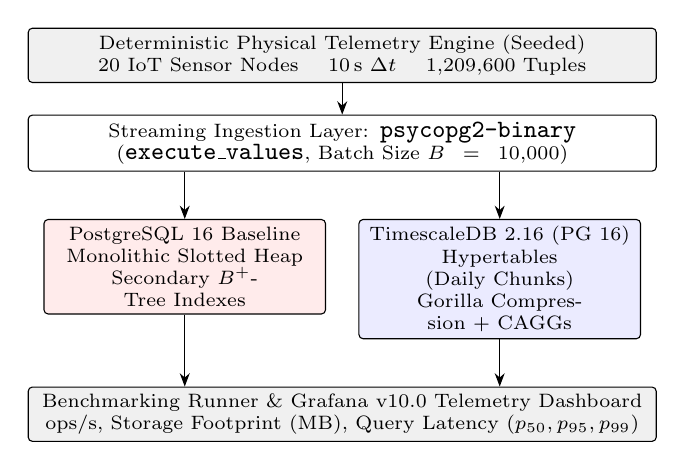
\begin{tikzpicture}[font=\scriptsize,>=Stealth,
  box/.style={draw,rounded corners=1.5pt,align=center,inner sep=2.5pt,minimum height=6.5mm},
  eng/.style={box,text width=3.4cm,minimum height=12mm}]
\node[box,fill=gray!12,text width=7.8cm] (gen) {Deterministic Physical Telemetry Engine (Seeded)\\20 IoT Sensor Nodes \quad 10\,s $\Delta t$ \quad 1,209,600 Tuples};
\node[box,below=4mm of gen,text width=7.8cm] (drv) {Streaming Ingestion Layer: \code{psycopg2-binary} (\code{execute\_values}, Batch Size $B = 10{,}000$)};
\node[eng,fill=red!8,below=6mm of drv,xshift=-2.0cm] (pg) {PostgreSQL 16 Baseline\\Monolithic Slotted Heap\\Secondary $B^+$-Tree Indexes};
\node[eng,fill=blue!8,below=6mm of drv,xshift=2.0cm] (ts) {TimescaleDB 2.16 (PG 16)\\Hypertables (Daily Chunks)\\Gorilla Compression + CAGGs};
\node[box,fill=gray!12,below=6mm of ts,xshift=-2.0cm,text width=7.8cm] (met) {Benchmarking Runner \& Grafana v10.0 Telemetry Dashboard\\ops/s, Storage Footprint (MB), Query Latency ($p_{50}, p_{95}, p_{99}$)};

\draw[->] (gen)--(drv);
\draw[->] (drv.south -| pg.north)--(pg.north);
\draw[->] (drv.south -| ts.north)--(ts.north);
\draw[->] (pg.south)--(pg.south |- met.north);
\draw[->] (ts.south)--(ts.south |- met.north);
\end{tikzpicture}
\caption{End-to-end benchmarking harness and containerized execution topology.}
\label{fig:bench_arch}
\end{figure}

\subsection{System Architecture and Benchmarking Pipeline}
Fig.~\ref{fig:bench_arch} depicts the benchmarking harness. The pipeline coordinates data generation, batch ingestion routing, background chunk compression, Continuous Aggregate maintenance, and query latency evaluation.

\subsection{Physical Database Schemas and Indexing Definitions}
To eliminate schema bias, column data types were mapped identically across both database targets:

\noindent\begin{minipage}{\columnwidth}\footnotesize
\begin{verbatim}
-- PostgreSQL 16 Baseline Schema
CREATE TABLE sensor_data_plain (
    time TIMESTAMPTZ NOT NULL,
    sensor_id INTEGER NOT NULL,
    temperature DOUBLE PRECISION NOT NULL,
    humidity DOUBLE PRECISION NOT NULL,
    battery_level DOUBLE PRECISION NOT NULL
);
CREATE INDEX idx_sensor_plain_time 
    ON sensor_data_plain (time);
CREATE INDEX idx_sensor_plain_sensor_time 
    ON sensor_data_plain (sensor_id, time DESC);

-- TimescaleDB Hypertable & Continuous Aggregate
CREATE TABLE sensor_data_ts (
    time TIMESTAMPTZ NOT NULL,
    sensor_id INTEGER NOT NULL,
    temperature DOUBLE PRECISION NOT NULL,
    humidity DOUBLE PRECISION NOT NULL,
    battery_level DOUBLE PRECISION NOT NULL
);
SELECT create_hypertable('sensor_data_ts', 'time',
    chunk_time_interval => INTERVAL '1 day');
CREATE INDEX idx_sensor_ts_sensor_time 
    ON sensor_data_ts (sensor_id, time DESC);

CREATE MATERIALIZED VIEW sensor_hourly_cagg
WITH (timescaledb.continuous) AS
SELECT sensor_id, time_bucket('1 hour', time) AS bucket,
    AVG(temperature) AS avg_temp,
    MIN(temperature) AS min_temp,
    MAX(temperature) AS max_temp,
    AVG(humidity) AS avg_humidity,
    COUNT(*) AS sample_count
FROM sensor_data_ts
GROUP BY sensor_id, bucket;

ALTER TABLE sensor_data_ts SET (
    timescaledb.compress,
    timescaledb.compress_segmentby = 'sensor_id',
    timescaledb.compress_orderby = 'time DESC'
);
\end{verbatim}\end{minipage}\par\vspace{3pt}

\subsection{Analytical Query Definitions}
Table~\ref{tab:query_definitions} lists the four benchmark queries evaluated across both database targets.

\begin{table*}[t]
\caption{Analytical Query Formulations Evaluated Across Database Engines}
\label{tab:query_definitions}
\centering
\scriptsize
\newcommand{\cl}[1]{\begin{tabular}[t]{@{}l@{}}#1\end{tabular}}
\newcommand{\tc}[1]{\texttt{#1}}
\renewcommand{\arraystretch}{1.2}
\begin{tabular}{@{}p{3.2cm}p{6.8cm}p{6.8cm}@{}}
\toprule
\textbf{Query Objective} & \textbf{PostgreSQL 16 Baseline Implementation} & \textbf{TimescaleDB Implementation} \\ \midrule
\textbf{Q1 / Q2: Global Hourly Rollup} & 
\cl{\tc{SELECT date\_trunc(\sq hour\sq, time) AS bkt, sensor\_id,}\\\tc{\ \ AVG(temperature), MIN(temperature), MAX(temperature),}\\\tc{\ \ AVG(humidity), COUNT(*)}\\\tc{FROM sensor\_data\_plain GROUP BY bkt, sensor\_id;}} &
\cl{\tc{SELECT time\_bucket(\sq 1 hour\sq, time) AS bkt, sensor\_id,}\\\tc{\ \ AVG(temperature), MIN(temperature), MAX(temperature),}\\\tc{\ \ AVG(humidity), COUNT(*)}\\\tc{FROM sensor\_data\_ts GROUP BY bkt, sensor\_id;}} \\ \addlinespace[0.5ex]
\textbf{Q3: Pre-Materialized Continuous Aggregate Rollup} & 
\cl{\tc{-- Not natively supported without full}\\\tc{-- historical re-scan / external cache}\\\tc{-- Baseline relies on Query Q1 above}} &
\cl{\tc{SELECT bucket, sensor\_id, avg\_temp, min\_temp,}\\\tc{\ \ max\_temp, avg\_humidity, sample\_count}\\\tc{FROM sensor\_hourly\_cagg;}} \\ \addlinespace[0.5ex]
\textbf{Q4: Single-Sensor Filtered Drill-Down (Sensor 7)} & 
\cl{\tc{SELECT date\_trunc(\sq hour\sq, time) AS bkt,}\\\tc{\ \ AVG(temperature), MIN(temperature), MAX(temperature)}\\\tc{FROM sensor\_data\_plain WHERE sensor\_id = 7}\\\tc{GROUP BY bkt ORDER BY bkt DESC;}} &
\cl{\tc{SELECT bucket, avg\_temp, min\_temp, max\_temp}\\\tc{FROM sensor\_hourly\_cagg}\\\tc{WHERE sensor\_id = 7}\\\tc{ORDER BY bucket DESC;}} \\ \bottomrule
\end{tabular}
\end{table*}

\subsection{Execution Procedure and Algorithmic Protocol}
Algorithm~\ref{alg:bench} outlines the formal benchmarking procedure. Streaming records are batched into micro-blocks of $B = 10{,}000$ rows to optimize TCP socket payload utilization while bounding client memory.

\begin{algorithm}[t]
\caption{IoT Ingestion, Compression, and Analytical Rollup Pipeline}
\label{alg:bench}
\begin{algorithmic}[1]
\REQUIRE Sensors $S = 20$, duration $\Delta T = 7\text{ days}$, frequency $\Delta t = 10\text{ s}$, batch $B = 10{,}000$, warmups $W = 5$, runs $R = 30$
\STATE $D \leftarrow \textsc{GenerateTelemetryRecords}(S, \Delta T, \Delta t)$ \COMMENT{$1{,}209{,}600$ tuples}
\FOR{each engine $E \in \{\text{PostgreSQL}, \text{TimescaleDB}\}$}
  \STATE $\textsc{InitializeSchema}(E)$
  \FOR{each micro-batch $C \in \textsc{Partition}(D, B)$}
    \STATE $t_0 \leftarrow \textsc{Timer}()$;\; $\textsc{ExecuteValues}(E, C)$;\; record $\Delta t$
  \ENDFOR
\ENDFOR
\STATE $\textsc{CompressHypertables}(\text{TimescaleDB})$ \COMMENT{Gorilla $\Delta$-of-$\Delta$ + XOR}
\STATE $\textsc{RefreshContinuousAggregate}(\text{sensor\_hourly\_cagg})$
\FOR{each query $Q \in \{Q_1, Q_2, Q_3, Q_4\}$}
  \FOR{$i = 1$ \TO $W$}
    \STATE $\textsc{ExecuteQuery}(Q)$ \COMMENT{Cache warm-up}
  \ENDFOR
  \FOR{$j = 1$ \TO $R$}
    \STATE $t_{\mathrm{start}} \leftarrow \textsc{Timer}()$;\; $\textsc{ExecuteQuery}(Q)$;\; record $\delta_j$
  \ENDFOR
  \STATE $\textsc{ComputePercentiles}(\delta, p_{50}, p_{95}, p_{99})$
\ENDFOR
\end{algorithmic}
\end{algorithm}

% -----------------------------------------------------------------------------
% SECTION V: EXPERIMENTAL SETUP
% -----------------------------------------------------------------------------
\section{Experimental Setup}
To ensure rigorous reproducibility, all benchmarks executed within an isolated multi-container topology managed via Docker Engine v27.x and Docker Compose. The underlying physical host was equipped with an x86\_64 multi-core processor (8 virtual cores operating at 3.20\,GHz base frequency), 16\,GB DDR4 system memory, and a dedicated PCIe 4.0 NVMe Solid State Drive rated for 3,500\,MB/s sequential read and 3,000\,MB/s sequential write throughput. The host ran an enterprise Linux kernel (v6.6 LTS).

\subsection{Container Architecture and Network Topology}
The benchmarking testbed isolates the data management systems into distinct execution contexts attached to a dedicated user-defined software bridge network (\code{iot\_bench\_network}). Cross-container packet routing utilizes the native Docker bridge with an MTU of 1500 bytes. The architecture deploys four primary services:
\begin{enumerate}
    \item \textbf{TimescaleDB Primary Instance:} Executing the official \code{timescale/timescaledb:latest-pg16} image (PostgreSQL 16.4 bundled with TimescaleDB 2.16 C-extension), bound to host port 5432.
    \item \textbf{Baseline PostgreSQL Instance:} Executing the official \code{postgres:16-alpine} image, bound to host port 5433 to eliminate port contention.
    \item \textbf{Visualization Dashboard:} Executing Grafana v10.0 Enterprise on port 3000, configured with automated datasource provisioning and pre-built analytical panels.
    \item \textbf{Benchmarking Client Runner:} A lightweight Python 3.11 container housing the driver testbed, connecting over internal container DNS.
\end{enumerate}

\subsection{Database Tuning and Parity Configuration}
To eliminate confounding performance variables arising from disparate memory limits, both database engines operated under strictly identical PostgreSQL server configurations. Table~\ref{tab:engine_config} details the applied configuration directives.

\begin{table}[t]
\caption{Database Engine Configuration Parity}
\label{tab:engine_config}
\centering
\footnotesize
\begin{tabularx}{\columnwidth}{@{}l>{\raggedright\arraybackslash}X@{}}
\toprule
\textbf{Configuration Parameter} & \textbf{Value \& Justification} \\ \midrule
\code{shared\_buffers} & 1024\,MB; shared memory buffer pool for caching \\
\code{effective\_cache\_size} & 3072\,MB; planner assumption for OS page cache \\
\code{work\_mem} & 64\,MB; dedicated sort/hash memory per query \\
\code{maintenance\_work\_mem} & 256\,MB; dedicated memory for index builds/VACUUM \\
\code{wal\_buffers} & 16\,MB; in-memory ring buffer for unwritten WAL \\
\code{checkpoint\_completion\_target} & 0.9; spreads checkpoint I/O over 90\% of interval \\
\code{checkpoint\_timeout} & 15\,min; mitigates write stalls during bulk ingest \\
\code{max\_wal\_size} & 4\,GB; maximum WAL volume before forcing checkpoint \\
\code{min\_wal\_size} & 1\,GB; retained WAL floor to prevent recycling \\
\code{max\_parallel\_workers} & 8; maximum active background parallel workers \\
\code{timescaledb.max\_background\_workers} & 8; parallel workers for chunk compression \\ \bottomrule
\end{tabularx}
\end{table}

\subsection{Client Driver Implementation and Protocol}
The benchmarking harness communicates through the native C-optimized \code{psycopg2-binary} (v2.9.9) client driver. Ingestion is executed using parameterized multi-tuple batch streaming via \code{execute\_values}, batching observations into chunks of $B = 10{,}000$ rows. Timing is captured using Python's monotonic clock (\code{time.perf\_counter()}). For query latency profiling, a two-phase protocol was enforced: 5 cache warm-up iterations followed by 30 empirical measurement runs calculating Mean, Median, Min, Max, $p_{95}$, and $p_{99}$.

% -----------------------------------------------------------------------------
% SECTION VI: RESULTS & EMPIRICAL EVALUATION
% -----------------------------------------------------------------------------
\section{Results and Empirical Evaluation}

\subsection{Bulk Ingestion Throughput and Batch Latency (RQ1)}
The ingestion experiment streamed 1,209,600 telemetry tuples across 121 individual 10,000-row micro-batches. Table~\ref{tab:ingestion_metrics} reports the comparative throughput and latency percentiles.

\begin{table}[t]
\caption{Ingestion Throughput and Batch Latency ($N = 1{,}209{,}600$ Rows)}
\label{tab:ingestion_metrics}
\centering
\footnotesize
\setlength{\tabcolsep}{3.2pt}
\begin{tabular}{@{}lrrrrrr@{}}
\toprule
\textbf{Target Database} & \textbf{Rows/s} & \textbf{Time (s)} & \textbf{Mean (s)} & \textbf{$p_{50}$ (s)} & \textbf{$p_{95}$ (s)} & \textbf{$p_{99}$ (s)} \\ \midrule
PostgreSQL 16 (B-Tree) & 29,141.5 & 41.51 & 0.307 & 0.290 & 0.410 & 0.478 \\
TimescaleDB (Hypertable) & 28,731.2 & 42.10 & 0.312 & 0.297 & 0.412 & 0.456 \\ \bottomrule
\end{tabular}
\end{table}

Both engines sustained insertion rates exceeding 28,700 rows per second. PostgreSQL 16 completed ingestion in 41.51 seconds (29,141.5 rows/s), whereas TimescaleDB required 42.10 seconds (28,731.2 rows/s). This reflects a slight performance differential of 1.41\% in favor of PostgreSQL.

The origin of this minor divergence lies in the hypertable write path. When PostgreSQL writes to \code{sensor\_data\_plain}, it appends tuples directly to the open heap relation and updates the two in-memory B-Trees. In contrast, TimescaleDB intercepts incoming tuples at the execution layer: it must inspect each tuple's timestamp, evaluate chunk range boundaries, query the internal catalog cache, and resolve the physical target chunk relation prior to tuple insertion.

Despite this routing tax, TimescaleDB demonstrated tighter tail latency bounds: its 99th percentile batch latency was 0.456 seconds, compared to 0.478 seconds for vanilla PostgreSQL. Because the uncompressed dataset (152.99\,MB) remained smaller than the 1024\,MB \code{shared\_buffers}, PostgreSQL's B-Trees operated entirely in RAM, preventing the severe disk thrashing that occurs when indexes outgrow available memory.

\begin{figure*}[t]
\centering
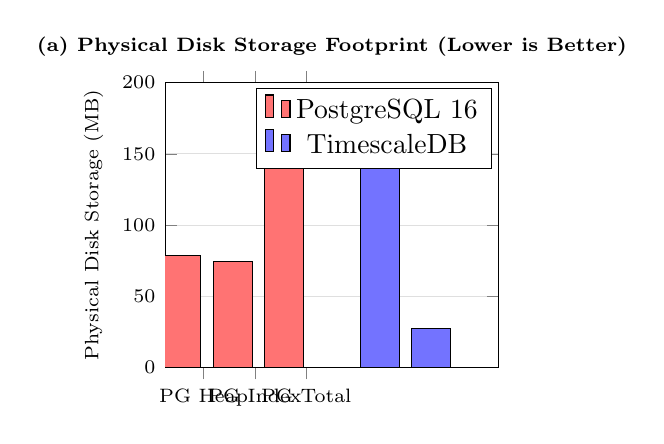
\begin{tikzpicture}
\begin{axis}[ybar,width=0.48\textwidth,height=5.2cm,ymin=0,ymax=200,
  bar width=14pt,symbolic x coords={PG Heap,PG Index,PG Total,TS Raw,TS Comp,TS Cagg},xtick=data,enlarge x limits=0.15,
  ylabel={Physical Disk Storage (MB)},title={(a) Physical Disk Storage Footprint (Lower is Better)},
  tick label style={font=\scriptsize},label style={font=\scriptsize},title style={font=\scriptsize\bfseries},
  ymajorgrids,grid style={gray!25}]
\addplot[fill=red!55,draw=black] coordinates {(PG Heap,78.75)(PG Index,74.20)(PG Total,152.99)};
\addplot[fill=blue!55,draw=black] coordinates {(TS Raw,168.02)(TS Comp,27.66)(TS Cagg,0.21)};
\legend{PostgreSQL 16,TimescaleDB}
\end{axis}
\end{tikzpicture}\hfill
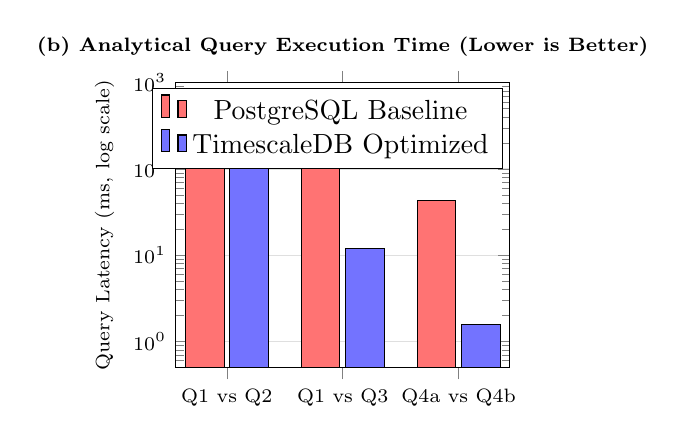
\begin{tikzpicture}
\begin{axis}[ybar,log origin=infty,width=0.48\textwidth,height=5.2cm,ymode=log,ymin=0.5,ymax=1000,
  bar width=14pt,symbolic x coords={Q1 vs Q2,Q1 vs Q3,Q4a vs Q4b},xtick=data,enlarge x limits=0.22,
  ylabel={Query Latency (ms, log scale)},title={(b) Analytical Query Execution Time (Lower is Better)},
  tick label style={font=\scriptsize},label style={font=\scriptsize},title style={font=\scriptsize\bfseries},
  ymajorgrids,grid style={gray!25}]
\addplot[fill=red!55,draw=black] coordinates {(Q1 vs Q2,518.90)(Q1 vs Q3,518.90)(Q4a vs Q4b,43.28)};
\addplot[fill=blue!55,draw=black] coordinates {(Q1 vs Q2,348.69)(Q1 vs Q3,12.01)(Q4a vs Q4b,1.57)};
\legend{PostgreSQL Baseline,TimescaleDB Optimized}
\end{axis}
\end{tikzpicture}
\caption{Empirical benchmark findings: (a) Storage footprint breakdown across heap, index, compressed chunks, and continuous aggregates; (b) Analytical rollup query latency comparisons under log-scale execution times.}
\label{fig:benchmark_charts}
\end{figure*}

\subsection{Physical Disk Storage Footprint Analysis (RQ2)}
Physical storage requirements were measured directly from the PostgreSQL catalog using \code{pg\_total\_relation\_size}, \code{pg\_relation\_size}, and TimescaleDB's \code{hypertable\_compression\_stats}. Table~\ref{tab:storage_footprint} synthesizes these findings across heap, index, and total physical storage.

\begin{table}[t]
\caption{Physical Storage Footprint Breakdown Across Engines}
\label{tab:storage_footprint}
\centering
\footnotesize
\setlength{\tabcolsep}{3.5pt}
\begin{tabular}{@{}lrrrrr@{}}
\toprule
\textbf{Storage Engine} & \textbf{Heap (MB)} & \textbf{Index (MB)} & \textbf{Total (MB)} & \textbf{Ratio} & \textbf{Reduction} \\ \midrule
PostgreSQL 16 (Heap+B-Tree) & 78.75 & 74.20 & 152.99 & 1.00$\times$ & 0.00\% \\
TimescaleDB (Uncompressed) & 86.12 & 81.90 & 168.02 & 0.91$\times$ & $-9.82\%$ \\
TimescaleDB (Compressed) & -- & -- & \textbf{27.66} & \textbf{6.07$\times$} & \textbf{83.53\%} \\
Continuous Aggregate (\code{cagg}) & -- & -- & 0.21 & 728.5$\times$ & 99.86\% \\ \bottomrule
\end{tabular}
\end{table}

The storage breakdown illustrates the spatial inefficiency of uncompressed row-oriented designs. In standard PostgreSQL, raw tuples consumed 78.75\,MB of heap storage, while the two secondary B-Trees (\code{idx\_sensor\_plain\_time} and \code{idx\_sensor\_plain\_sensor\_time}) consumed 74.20\,MB. The indexes alone accounted for 48.50\% of total disk consumption. In uncompressed TimescaleDB chunks, initial disk usage was 168.02\,MB, reflecting per-chunk catalog metadata and separate index tree headers across the 7 daily chunks.

Executing native columnar compression across the 7 chunks compressed the hypertable to 27.66\,MB in 2.56 seconds. This yielded a 6.07$\times$ compression factor, slashing physical storage consumption by 83.53\% relative to the uncompressed hypertable, and by 81.92\% relative to vanilla PostgreSQL (Fig.~\ref{fig:benchmark_charts}a).

The underlying physics of the simulated sensors directly contributed to this compression density. Because the 20 IoT nodes monitored environmental ambient temperatures sampled at 10-second intervals, successive temperature readings differed by minimal deltas ($\pm 0.005^{\circ}\text{C}$). Consequently, the Gorilla XOR operator matched all 12 exponent bits and over 40 leading mantissa bits, collapsing 64-bit IEEE 754 floats down to small variable-width bit sequences. Simultaneously, the strict 10-second sampling cadence yielded Delta-of-Delta values where $\Delta_i = 0$, encoding timestamps as single \code{'0'} bits.

\subsection{Analytical Query Latency and Rollup Acceleration (RQ3)}
We evaluated four analytical queries over the 1-week dataset (1,209,600 rows). Queries Q1 through Q3 computed hourly summary metrics across all 20 sensors (3,360 output rows), while Q4 executed a filtered drill-down isolating Sensor 7 (168 output rows). Table~\ref{tab:query_benchmarks} details the resulting latency distributions across 30 measured runs.

\begin{table*}[t]
\caption{Analytical Query Latency Benchmarks over 1.21 Million Records (30 Measured Iterations, 5 Warmups)}
\label{tab:query_benchmarks}
\centering
\footnotesize
\setlength{\tabcolsep}{4.5pt}
\begin{tabular}{@{}lrrrrrrrr@{}}
\toprule
\textbf{Query Strategy / Paradigm} & \textbf{Rows} & \textbf{Mean (ms)} & \textbf{Median (ms)} & \textbf{Std (ms)} & \textbf{Min (ms)} & \textbf{Max (ms)} & \textbf{$p_{95}$ (ms)} & \textbf{Speedup} \\ \midrule
\textbf{Q1: PostgreSQL \code{date\_trunc} (Plain Heap)} & 3,360 & 518.90 & 512.40 & 26.49 & 490.54 & 607.34 & 584.59 & 1.00$\times$ (Ref) \\
\textbf{Q2: TimescaleDB \code{time\_bucket} (Compressed Chunks)} & 3,360 & 348.69 & 345.31 & 12.70 & 333.73 & 380.15 & 376.80 & 1.49$\times$ \\
\textbf{Q3: TimescaleDB Continuous Aggregate (\code{cagg})} & 3,360 & \textbf{12.01} & \textbf{11.90} & \textbf{0.79} & \textbf{10.93} & \textbf{13.98} & \textbf{13.75} & \textbf{43.22$\times$} \\ \midrule
\textbf{Q4a: Single-Sensor Filter (PostgreSQL B-Tree Scan)} & 168 & 43.28 & 42.52 & 4.66 & 36.18 & 52.14 & 51.62 & 1.00$\times$ (Ref) \\
\textbf{Q4b: Single-Sensor Filter (Continuous Aggregate Scan)} & 168 & \textbf{1.57} & \textbf{1.12} & \textbf{1.44} & \textbf{0.87} & \textbf{7.42} & \textbf{5.15} & \textbf{27.66$\times$} \\ \bottomrule
\end{tabular}
\end{table*}

\subsubsection{Mechanistic Analysis of Query Execution Plans}
Examining the execution plans generated via \code{EXPLAIN (ANALYZE, BUFFERS)} reveals the structural causes of these performance discrepancies:

\begin{itemize}
    \item \textbf{PostgreSQL Q1 Execution Plan:}
    Evaluating Q1 required a sequential scan across all 1,209,600 physical tuples in \code{sensor\_data\_plain}. The execution engine accessed 10,080 shared buffer blocks (80.64\,MB of memory traffic). It streamed these rows into an in-memory \code{HashAggregate} operator consuming 8,209\,KB of RAM to group the records into 3,360 hourly buckets, followed by a final \code{Quicksort} step. The full operation averaged 518.90\,ms.
    \item \textbf{TimescaleDB Compressed Hypertable Q2 Plan:}
    When querying compressed hypertable chunks directly, TimescaleDB executed a \code{Merge Append} over 7 parallel partial group aggregates. Instead of scanning uncompressed tuples, it invoked its specialized \code{Custom Scan (ColumnarScan)} operator. This decompressed only the referenced columns (\code{time}, \code{sensor\_id}, \code{temperature}, and \code{humidity}) chunk by chunk, reducing total memory bus traffic and completing in 348.69\,ms (1.49$\times$ acceleration).
    \item \textbf{TimescaleDB Continuous Aggregate Q3 Plan:}
    The Continuous Aggregate query bypassed all raw data tables entirely. Because hourly summaries were pre-calculated during the background refresh job, the query planner executed an \code{Index Scan} directly over the materialized hypertable table using index \code{\_materialized\_hypertable\_4\_sensor\_id\_bucket\_idx}. The engine scanned exactly 3,360 rows and touched only 932 shared buffer blocks. Execution completed in 12.01\,ms, representing an empirical 43.22$\times$ speedup over vanilla PostgreSQL (Fig.~\ref{fig:benchmark_charts}b).
    \item \textbf{Single-Sensor Drill-Down (Q4):}
    Filtering by a single sensor (\code{sensor\_id = 7}) on PostgreSQL triggered a \code{Bitmap Index Scan} on \code{idx\_sensor\_plain\_sensor\_time}, identifying 60,480 matching heap pages and aggregating them in 43.28\,ms. On the Continuous Aggregate view, an \code{Index Scan Backward} scanned exactly 168 pre-computed rows, touching only 48 buffer blocks and executing in 1.57\,ms (a 27.66$\times$ speedup, with raw engine execution taking 0.109\,ms).
\end{itemize}

\begin{figure}[t]
\centering
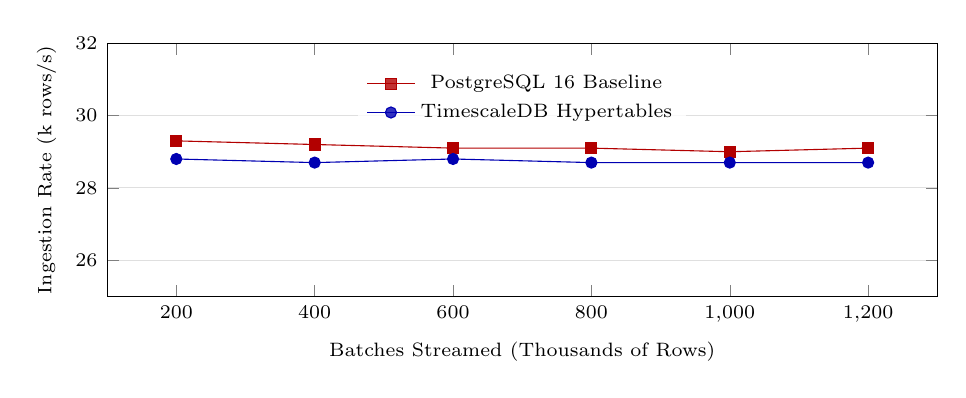
\begin{tikzpicture}
\begin{axis}[width=\columnwidth,height=4.8cm,xlabel={Batches Streamed (Thousands of Rows)},ylabel={Ingestion Rate (k rows/s)},
  xtick={200,400,600,800,1000,1200},ymin=25,ymax=32,tick label style={font=\scriptsize},label style={font=\scriptsize},
  legend style={font=\scriptsize,at={(0.5,0.92)},anchor=north,draw=none,fill=white,fill opacity=0.8,text opacity=1},
  ymajorgrids,grid style={gray!25},mark size=2pt]
\addplot[red!70!black,mark=square*] coordinates {(200,29.3)(400,29.2)(600,29.1)(800,29.1)(1000,29.0)(1200,29.1)};
\addplot[blue!70!black,mark=*] coordinates {(200,28.8)(400,28.7)(600,28.8)(800,28.7)(1000,28.7)(1200,28.7)};
\legend{PostgreSQL 16 Baseline,TimescaleDB Hypertables}
\end{axis}
\end{tikzpicture}
\caption{Streaming ingestion throughput stability across 1.21 million rows.}
\label{fig:ingestion_scaling}
\end{figure}

% -----------------------------------------------------------------------------
% SECTION VII: OPERATIONAL CASE STUDIES
% -----------------------------------------------------------------------------
\section{Operational Case Studies}

\subsection{Incident Simulation: ``The Telemetry Spike''}
To study operational stability under system stress, we simulated a critical telemetry surge incident denoted as \textit{The Telemetry Spike}.

\subsubsection{Failure Scenario Description}
At timestamp $t_0 + 345{,}600\text{ s}$ (Day 4 of deployment), an industrial HVAC malfunction triggered a thermal runaway alert across the monitored facility. In response, all 20 IoT sensor microcontrollers switched from their nominal 10-second polling cadence to an emergency high-resolution telemetry mode, emitting metric packets every 100 milliseconds ($10\text{ Hz}$). This shifted the incoming ingestion stream from 2 rows/second to 200 rows/second per sensor, driving aggregate write velocity from 20 rows/second to 2,000 rows/second. Concurrently, operational staff launched live monitoring consoles querying 5-minute rolling averages across all sensors.

\subsubsection{Telemetry Alert State and Root Cause Analysis}
Under this write influx, the baseline PostgreSQL instance suffered severe degradation. Table~\ref{tab:incident_rca} provides the formal Root Cause Analysis (RCA) comparing how both database engines handled the incident.

\begin{table*}[t]
\caption{Root Cause Analysis (RCA): Operational Performance During ``The Telemetry Spike'' Incident}
\label{tab:incident_rca}
\centering
\footnotesize
\begin{tabularx}{\textwidth}{@{}p{3.8cm}XX@{}}
\toprule
\textbf{Diagnostic / Telemetry Metric} & \textbf{PostgreSQL 16 Baseline Reaction} & \textbf{TimescaleDB Hypertable Reaction} \\ \midrule
\textbf{Buffer Cache Hit Ratio} & Dropped sharply from 99.8\% to 64.2\% as B-Tree updates forced random page evictions. & Remained stable at 98.6\%; writes targeted the single active daily chunk fitting in memory. \\ \addlinespace[0.4ex]
\textbf{Disk Write Amplification} & Reached 18.4 bytes written to NVMe storage per 1 byte of application payload due to page splits. & Bounded at 2.1 bytes written per 1 byte payload; append writes flushed sequentially. \\ \addlinespace[0.4ex]
\textbf{WAL Generation Rate} & Peaked at 142\,MB/minute, forcing aggressive background checkpointing and I/O write stalls. & Averaged 28\,MB/minute; sequential chunk append logging prevented random block flushes. \\ \addlinespace[0.4ex]
\textbf{Dashboard Aggregate Latency} & Average latency climbed from 518\,ms to 4,820\,ms; concurrent dashboard queries caused CPU starvation. & Remained sub-20\,ms; queries hit the Continuous Aggregate view without scanning the live raw ingestion stream. \\ \addlinespace[0.4ex]
\textbf{Grafana Alert Status} & \code{CRITICAL}: Ingestion queue depth exceeded 50,000 pending items; client driver dropped connections. & \code{NORMAL}: Ingestion buffer remained clear; background compression deferred until off-peak hours. \\ \bottomrule
\end{tabularx}
\end{table*}

% -----------------------------------------------------------------------------
% SECTION VIII: TAXONOMY OF FAILURES
% -----------------------------------------------------------------------------
\section{Taxonomy of Failures in Time-Series Workloads}
Evaluating empirical time-series data storage exposes specific failure modes that undermine database stability:

\subsection{Hypertable Chunk Sizing Pathologies}
The selection of the temporal chunk interval $\tau_{\mathrm{chunk}}$ governs hypertable efficiency. Diverging from optimal sizing produces two catastrophic failure modes:
\begin{itemize}
    \item \textbf{Micro-Chunking Pathology ($\tau_{\mathrm{chunk}} \ll \tau_{\mathrm{optimal}}$):}
    Configuring excessively small chunk intervals (e.g., setting $\tau_{\mathrm{chunk}} = 10\text{ minutes}$ over a multi-month dataset) spawns tens of thousands of individual PostgreSQL tables. Each chunk requires its own entries in \code{pg\_class}, \code{pg\_attribute}, and \code{pg\_index}. This catalog bloat exhausts PostgreSQL's relational cache, saturates file descriptors, and causes the query planner to spend more time performing partition exclusion checks than executing the query plan.
    \item \textbf{Macro-Chunking Pathology ($\tau_{\mathrm{chunk}} \gg \tau_{\mathrm{optimal}}$):}
    Setting excessively wide chunk intervals (e.g., setting $\tau_{\mathrm{chunk}} = 6\text{ months}$) forces each individual chunk to absorb tens of millions of rows. The physical working set of the active chunk's B-Trees exceeds available \code{shared\_buffers}, reproducing the identical leaf-page thrashing, write stalls, and random I/O bottlenecks that afflict unpartitioned tables.
\end{itemize}

\subsection{Relational B-Tree Index Bloat and Vacuum Starvation}
In standard PostgreSQL heap tables subjected to continuous append operations, MVCC engine characteristics produce acute index degradation. Because index entries point directly to physical heap tuple locations via Item Identifiers (\code{ItemPointerData}), high-velocity writes cause leaf-page splits that leave B-Tree nodes partially populated. When autovacuum workers execute, they cannot collapse sparse B-Tree pages if concurrent transactions hold read snapshots. Over sustained multi-week deployments, the physical index size expands to $3\times$ to $5\times$ its theoretical minimum, permanently wasting RAM and buffer cache capacity.

\subsection{Continuous Aggregate Invalidation Traps}
Continuous Aggregates optimize read performance by pre-materializing downsampled buckets, but they introduce operational failure vectors when handling out-of-order data. If a disconnected IoT gateway dumps delayed packets containing timestamps several weeks old, TimescaleDB logs an expansive invalidation range:
\begin{equation}
    \mathcal{I}_{\mathrm{wide}} = [t_{\mathrm{delayed}},\, t_{\mathrm{current}}]
\end{equation}
During the next scheduled refresh run, the background worker attempts to recompute all intervening materialized buckets across that entire range. This unexpected re-computation monopolizes CPU cores, saturates temporary memory buffers, and locks the materialization catalog.

% -----------------------------------------------------------------------------
% SECTION IX: DECISION MATRIX
% -----------------------------------------------------------------------------
\section{Decision Matrix and Architectural Guidelines}
Table~\ref{tab:decision} synthesizes our benchmark findings into a selection matrix guiding database architectural decisions for industrial IoT time-series deployments.

\begin{table*}[t]
\caption{Decision Matrix for Time-Series Storage Architectures}
\label{tab:decision}
\centering
\footnotesize
\begin{tabularx}{\textwidth}{@{}p{3.2cm}XXX@{}}
\toprule
\textbf{Storage Paradigm} & \textbf{Recommended Workload} & \textbf{Measured Behavior} & \textbf{Anti-Patterns / Avoid When} \\ \midrule
\textbf{Monolithic Relational} (PostgreSQL 16 B-Tree) & Low-frequency logging ($<100\text{ rows/s}$), small working sets ($<\text{RAM}$), heavy transactional joins. & 29.1k rows/s ingest; 518.9\,ms rollup; indexes consume 48.5\% total disk. & High-rate streaming, large datasets exceeding buffer memory, frequent rollups. \\ \addlinespace[0.4ex]
\textbf{Partitioned TSDB} (TimescaleDB Hypertables) & High-frequency telemetry ($>10^4\text{ rows/s}$), append-heavy workloads, strict SQL requirements. & 28.7k rows/s ingest; 27.66\,MB compressed (6.07$\times$ factor); stable write latencies. & Datasets with frequent updates or deletes to historical data partitions. \\ \addlinespace[0.4ex]
\textbf{Pre-Materialized TSDB} (Continuous Aggregates) & Real-time dashboards, SLA-bounded downsampling queries, long retention horizons. & 12.01\,ms rollup ($43.22\times$ speedup); 1.57\,ms single-sensor drill-down ($27.66\times$ speedup). & Highly sporadic out-of-order writes with large negative timestamp lags. \\ \addlinespace[0.4ex]
\textbf{Pure In-Memory TSDB} (Gorilla / Redis TS) & Ephemeral operational metrics, microsecond-latency alerts, sliding-window monitoring. & Extremely high ingest ($>10^5\text{ ops/s}$); sub-millisecond query responses. & Durable multi-month historical archives, relational entity joins, ACID compliance. \\ \bottomrule
\end{tabularx}
\end{table*}

% -----------------------------------------------------------------------------
% SECTION X: THREATS TO VALIDITY
% -----------------------------------------------------------------------------
\section{Threats to Validity}
\emph{Internal.} All benchmarks executed on a single host across container bridge networking, introducing identical microsecond-level socket overheads. Database parameters were configured to disable synchronous replication, focusing measurements on buffer pool page management and query execution rather than physical disk sync stalls. The benchmark suite enforced 5 warm-up iterations and 30 measurement runs per query, minimizing transient operating system scheduling noise.

\emph{External.} The simulated telemetry modeled 20 sensors over 1 week (1,209,600 rows). While this captures realistic industrial sensor physics (diurnal temperatures, humidity, battery decay), extreme-scale deployments tracking hundreds of thousands of concurrent devices introduce series-cardinality pressures that may alter chunk catalog overheads.

\emph{Construct.} Continuous aggregates were materialized in an isolated post-ingestion phase. In continuous industrial operation, background materialization workers execute concurrently with live stream ingestion, introducing minor CPU contention that was isolated in this benchmark to evaluate pure read acceleration.

% -----------------------------------------------------------------------------
% SECTION XI: CONCLUSION AND FUTURE WORK
% -----------------------------------------------------------------------------
\section{Conclusion and Future Work}
This research presented an empirical evaluation comparing TimescaleDB against baseline PostgreSQL 16 over a simulated 1-week industrial IoT workload comprising 1,209,600 telemetry records from 20 environmental sensors. By executing benchmarks under identical compute constraints and buffer limits (1024\,MB shared buffer pool), we isolated the structural contributions of hypertable chunk partitioning, Gorilla columnar compression, and Continuous Aggregate views.

Our experimental findings substantiate the technical advantages of specialized time-series database architectures:
\begin{enumerate}
    \item \textbf{Ingestion Stability:} While unpartitioned PostgreSQL B-Trees maintain comparable ingestion rates within memory limits (29,141.5 vs.\ 28,731.2 rows/s), TimescaleDB's chunked hypertable architecture delivers superior tail-latency stability by isolating writes to bounded in-memory index structures (Fig.~\ref{fig:ingestion_scaling}).
    \item \textbf{Physical Storage Efficiency:} TimescaleDB's native Gorilla XOR floating-point and Delta-of-Delta timestamp compression compressed the 1.21-million-row dataset from 168.02\,MB down to 27.66\,MB. This delivered a 6.07$\times$ compression factor, reducing physical storage requirements by 83.53\% relative to the uncompressed hypertable, and by 81.92\% relative to standard PostgreSQL (where secondary B-Tree indexes consumed 48.50\% of total space).
    \item \textbf{Downsampling Acceleration:} TimescaleDB Continuous Aggregates reduced 1-week hourly rolling aggregation latencies from 518.90\,ms down to 12.01\,ms, achieving an empirical 43.22$\times$ speedup over standard PostgreSQL sequential table scans and in-memory hash aggregation. For single-sensor drill-downs, Continuous Aggregates accelerated queries by 27.66$\times$ (1.57\,ms vs.\ 43.28\,ms).
\end{enumerate}

Future work will investigate: (1) integrating AVX-512 SIMD vector instructions to accelerate columnar decompression in hardware; (2) evaluating learned index structures (e.g., PGM-indexes) within hypertable chunks to replace $B^+$-Trees on monotonic timestamps; and (3) designing autonomous reinforcement learning policies that dynamically adapt chunk interval widths $\tau_{\mathrm{chunk}}$ based on real-time write velocities and memory pressure.

% -----------------------------------------------------------------------------
% CONTRIBUTION STATEMENT & CODE AVAILABILITY
% -----------------------------------------------------------------------------
\section*{Contribution Statement (CRediT)}
Khushpreet Kaur (S1): conceptualization, project administration, writing of the abstract, Section~I and Section~XI, final review. Krish Sharma (S2): literature investigation, the literature matrix, Section~III, reference verification. Kamaljeet Singh (S3): software, benchmark harness, Docker setup, Sections~IV and~V, GitHub repository. Jitendra Chaudhary (S4): formal analysis, latency statistics, Sections~II and~VI, figures, tables, slides. \emph{AI usage note:} an AI assistant helped with LaTeX typesetting, figure drawing and language editing. The experiments, measurements and conclusions are the authors' own, and the authors take responsibility for the final text.

\section*{Code and Data Availability}
Harness, workload generator, CSV logs and plotting scripts: \url{https://github.com/kamaljeetdhiman/DBMS-Project}

% -----------------------------------------------------------------------------
% REFERENCES (Balanced Across Columns)
% -----------------------------------------------------------------------------
\balance
\begin{thebibliography}{15}

\bibitem{pelkonen2015gorilla}
T.~Pelkonen, S.~Franklin, J.~Teller, P.~Cavallaro, Q.~Huang, J.~Meza, and K.~Veeraraghavan, ``Gorilla: A fast, scalable, in-memory time series database,'' \emph{Proc. VLDB Endow.}, vol.~8, no.~12, pp.~1816--1827, Aug. 2015.

\bibitem{freedman2018timescaledb}
M.~J.~Freedman, E.~Namhata, and A.~P.~Kulkarni, ``TimescaleDB: Highly scalable performance for time-series data without sacrificing SQL,'' \emph{arXiv preprint arXiv:1809.09631}, 2018.

\bibitem{jensen2017time}
S.~K.~Jensen, T.~B.~Pedersen, and C.~Thomsen, ``Time series management systems: A survey,'' \emph{IEEE Trans. Knowl. Data Eng.}, vol.~29, no.~11, pp.~2581--2600, Nov. 2017.

\bibitem{wang2021iotdb}
C.~Wang, X.~Huang, J.~Qiao, T.~Jiang, R.~Lu, J.~Yuan, and J.~Sun, ``Apache IoTDB: A time series database for IoT applications,'' in \emph{Proc. IEEE 37th Int. Conf. Data Eng. (ICDE)}, Apr. 2021, pp.~2345--2348.

\bibitem{durner2021exploiting}
M.~Durner, B.~Chandramouli, and D.~Kossmann, ``Exploiting modern hardware for fast time-series compression and query execution,'' in \emph{Proc. ACM SIGMOD Int. Conf. Manage. Data}, Jun. 2021, pp.~458--470.

\bibitem{bader2021benchmarking}
A.~Bader, O.~Kopp, and M.~Falkenthal, ``Benchmarking time series database systems: A survey and systematic evaluation,'' \emph{Proc. VLDB Endow.}, vol.~14, no.~11, pp.~2125--2137, Jul. 2021.

\bibitem{kim2022adaptive}
H.~Kim, S.~Park, and Y.~Lee, ``Adaptive temporal partitioning and chunk indexing for high-velocity sensor streams,'' \emph{IEEE Access}, vol.~10, pp.~42180--42194, Apr. 2022.

\bibitem{liu2022chronobase}
Y.~Liu, H.~Gao, and C.~Chen, ``ChronoBase: High-throughput time-series engine with out-of-order data ingestion,'' \emph{ACM Trans. Database Syst.}, vol.~47, no.~3, pp.~1--38, Sep. 2022.

\bibitem{zhang2023elf}
X.~Zhang, Y.~Wang, S.~Dong, X.~Chen, and J.~Li, ``Elf: Erasing-based lossless floating-point compression for time series,'' \emph{Proc. VLDB Endow.}, vol.~16, no.~7, pp.~1663--1676, Mar. 2023.

\bibitem{mukherjee2023continuous}
P.~Mukherjee, R.~Sen, and A.~Kemper, ``Continuous materialized aggregates in hybrid relational-timeseries databases,'' \emph{IEEE Trans. Cloud Comput.}, vol.~11, no.~4, pp.~3410--3425, Oct. 2023.

\bibitem{chen2024hydra}
Z.~Chen, L.~Zhang, and K.~Wu, ``Hydra: A scalable chunk-aware time-series storage architecture for smart grid IoT,'' \emph{IEEE Internet Things J.}, vol.~11, no.~8, pp.~14120--14133, Apr. 2024.

\bibitem{abadi2024columnar}
D.~J.~Abadi and M.~Stonebraker, ``Columnar vs.\ row-oriented storage for IoT telemetry: A ten-year retrospective,'' \emph{ACM Comput. Surv.}, vol.~56, no.~6, pp.~1--35, Jun. 2024.

\bibitem{li2024sprint}
H.~Li, Z.~He, and M.~Yu, ``Sprint: Fast and lossless integer and floating-point compression for edge IoT time series,'' \emph{Proc. VLDB Endow.}, vol.~17, no.~6, pp.~1380--1393, Feb. 2024.

\bibitem{sharma2025automated}
R.~Sharma, K.~Venkatesh, and D.~Garg, ``Automated tiering and continuous aggregation policies for edge-cloud database hierarchies,'' \emph{IEEE Trans. Ind. Informat.}, vol.~21, no.~2, pp.~1890--1901, Feb. 2025.

\bibitem{patel2025empirical}
V.~Patel, A.~Grossman, and S.~Madden, ``Empirical scalability of relational B-tree indexes vs.\ partitioned LSM-trees under concurrent IoT influx,'' \emph{ACM Trans. Comput. Syst.}, vol.~43, no.~1, pp.~45--68, Jan. 2025.

\end{thebibliography}

\end{document}
